In order to evaluate if the approach to generate Linked Data from PSCs can improve the access to public procurement data 
exploiting the advantages of this initiative, two experiments have been designed:
\begin{enumerate}
 \item The first one checks if we can access more public procurement notices when the links between a PSC and the CPV are created. 
 The aim of this study is to compare the initial input vocabulary (containing only the CPV descriptors) and the final 
 input vocabulary (containing all descriptors that have linked to the CPV). Therefore if we extend the input vocabulary we can ease the access to 
 more public procurement notices because we can jump from any PSC to the CPV. In the same way if we need to make some kind of comparison 
 between systems working with different PSCs we can use the CPV as ``lingua franca''.
 
 \item The second study tries to exploit the semantic relationships between the CPV concepts to build a recommender of CPV codes for business users. 
 In order to make a empirical experiment we have used $11$ user queries and their translation into CPV codes made by the company ``Euroalert.net''.
\end{enumerate}

\subsection{Study 1}
\subsection{Research Design}
The purpose of this study is to compare the size of the initial input vocabulary for retrieving public procurement notices 
with regards to the final input vocabulary when links between a PSC and the CPV are created. The exploitation of these links can be used 
to build new SPARQL queries that can take advantage of Linked Data principles to provide a greater input vocabulary. Let's assume the following points about the 
public procurement notices and the PSCs used in this study:
\begin{itemize}
 \item All public procurement notices are always annotated by, at least, one CPV element.
 \item Each PSC is a controlled vocabulary. The CPV is a controlled vocabulary, $\mathcal{V}$, comprised of $10357$ elements/terms/codes.
 \item The public procurement notices is a RDF dataset, $\mathcal{D}$,
 Each document, $d \in \mathcal{D}$ is annotated, at least, using a CPV code, $v \in \mathcal{V}$. Thus, 
 if a query contains all elements, $v \in \mathcal{V}$, the entire dataset of notices will be retrieved.
\end{itemize}
Once these assumptions are defined, the gain of linking a new finite PSC to CPV can be calculated as follows:
\begin{itemize}
 \item The source controlled vocabulary, $\mathcal{V}_{psc}$, is comprised of \#$\mathcal{V}_{psc}$ elements.
 \item The linking of terms between a source vocabulary, $\mathcal{V}_{psc}$, and  a target vocabulary, $\mathcal{V}$ can be carried out in the next ways:
 \begin{enumerate}
  \item $1-1$ link, there are elements $v^k_{psc} \in \mathcal{V}_{psc}$ that are linked to only one element $v \in \mathcal{V}$.
  \item $1-n$ link, there are elements $v^k_{psc} \in \mathcal{V}_{psc}$ that are linked to some elements $v \in \mathcal{V}$ generating $K$ links.  
  \item The result of the previous operation generates links or pairs in the form $p_k=(v^k_{psc}, v^k)$ building a set of pairs $\mathcal{P}=\{p_1,p_2,...,p_k,p_n\}$. Taking into account this situation, 
  the initial vocabulary $V$ is increased in all elements $v^k_{psc} \in \mathcal{V}_{psc}$ that have a link to an element $v \in \mathcal{V}$. The new 
  derivate vocabulary $\mathcal{V'}_{psc}$ is a controlled vocabulary comprising all elements $v^k_{psc}: v^k_{psc} \in p_i$.
 \end{enumerate}
 
 \item The percentage of gain in terms of expressivity (number of elements to be used in queries) is related to the number of elements that enables go from $\mathcal{V}_{psc}$ to $\mathcal{V}$:	
 \begin{equation}\label{percentage}
  \%=100*(\frac{\#\mathcal{V'}_{psc} + \#\mathcal{V}}{\#\mathcal{V}}-1)
 \end{equation}
 
  As an example of this approach, two controlled vocabularies and a set of links/pairs are presented to calculate the gain in terms of expressivity:
  \begin{itemize}
  \item Let $\mathcal{V} = \{A, B, C, D, E\}$  and  $\mathcal{V}_{psc} = \{1, 2, 3\}$ the source and target controlled vocabularies.
  \item Let $P = \{ (A,1), (B,2), (C,1) (C,2) \}$ the set of links/pairs between $\mathcal{V}$ and $\mathcal{V}_{psc}$.
  \item Let $\mathcal{V'}_{psc} = \{ A, B, C \}$ the set of elements $v^k_{psc}: v^k_{psc} \in p_i$.
  \item Therefore, the new controlled vocabulary to query the dataset is comprised of $\{\mathcal{V_{psc}}\,\cup\,\mathcal{V'}_{psc}\}$ and the percentage of gain in terms of expressivity 
  according to the Equation~\ref{percentage} is:

  \begin{equation}
      \% = 100 * \{ \langle (3+3) / 3 \rangle -1 \} = 2-1 = 100 
  \end{equation}
      \item As a consequence the number of final terms to create queries is just two times than the initial set, increasing the expressivity in a $100\%$.
  \end{itemize}

 \item Finally, in this study, there is a specific scenario in which elements $v^k_{psc} \in \mathcal{V}_{psc}$ are not directly mapped to elements $v \in \mathcal{V}$ but 
 assuming that there are relations $r_k$  among elements $v^j_{psc}$  and $v^k_{psc}$ new links could emerge between $v^j_{psc}$ and $v$ through $r_k$. Nevertheless this 
 situation should be avoided in order to prevent an infinite and recursive linking process and keep the advantages of using finite controlled vocabularies, 
 e.g. in the ongoing example, Product Ontology (PO) is used as a bridge classification implying an infinite max gain ($\infty$).
 
\end{itemize}

\subsection{Sample}

The PSCs that have been selected to be promoted to RDF, see Table~\ref{table:pscs-ld}, are also used to check 
if the gain we can get through a direct link to the CPV 2008 or by means of creating a ``bridge link'' 
through the ProductOntology. The dataset $\mathcal{D}$ of public procurement notices contains $919341$ documents 
annotated with a total number of $1866367$ CPV codes (distinct $10062$).


\subsection{Results and Discussion}
Table~\ref{ganancia-terminos} presents the statistics of transforming each PSC as well as the number of terms that have linked to CPV 2008 and the gain (percentage) of 
new descriptors we can use to query the dataset. Following the same approach as in the previous example, the gain in terms 
of expressivity is calculated below:

\begin{itemize}
  \item Let $\mathcal{CPV}_{2003} = \{v^0_{cpv_{2003}}, v^1_{cpv_{2003}},...,v^n_{cpv_{2003}}\}$ and $\mathcal{CPV}_{2008} = \{v^0_{cpv_{2008}}, v^1_{cpv_{2008}},...,v^n_{cpv_{2008}}\}$ the source and target controlled vocabularies.
  \item Let $P = \{ (v^k_{cpv_{2003}},v^j_{cpv_{2008}})\}$ the set of links/pairs between $\mathcal{CPV}_{2003}$ and $\mathcal{CPV}_{2008}$.
  \item Let $\mathcal{CPV'}_{2008} = \{ v^k_{cpv_{2003}} \}$ the set of elements $v^k_{cpv_{2003}}: v^k_{cpv_{2003}} \in p_i$.
  \item Therefore, the new controlled vocabulary to query the dataset is comprised of $\{\mathcal{CPV}_{2008}\,\cup\,\mathcal{CPV'}_{2008}\}$ 
  and the percentage of gain in terms of expressivity according to the Equation~\ref{percentage} is:

  \begin{equation}
      \% = 100 * \{ \langle (462+10357) / 10357 \rangle -1 \} = 1,0446-1 = 4,46 
  \end{equation}
      
 \item As conclusion the real expressivity gain (in terms of descriptors to query a dataset) with regards to the initial set of $10357$ terms in CPV 2008 has been 
 increased in a $4.46$\% (462 new elements can be now used to build SPARQL queries). 

\end{itemize}

Taking into account the full results presented in Table~\ref{ganancia-terminos} the real expressivity gain (in terms of descriptors to query a dataset) 
with regards to the initial set of $10357$ terms in CPV 2008 has been increased in a $209,66$\% 
($21715$ new elements are part of the input vocabulary). Furthermore if the ProductOntology is used as a ``bridge'' the input vocabulary is then 
increased in a $285,66$\% ($29586$ new elements). Although this last approach shows a valuable increment in the number of linked elements 
it should be avoided due to the fact that more ``jumps'' between classifications imply necessarily less confidence in the mappings. Finally 
Figure~\ref{fig:results-3} presents the evolution of the input vocabulary when a new PSC is linked to the CPV 2008.

\begin{table}[!htb]
\scriptsize
\renewcommand{\arraystretch}{1.3}
\begin{center}
\begin{tabular}[c]{|p{2.2cm}|p{1.6cm}|p{1.8cm}|p{1.6cm}|p{1.6cm}|p{1.8cm}|p{1.6cm}|}
 
 \hline
  $\mathcal{V}_{psc}$ & $\#\mathcal{V}_{psc}$  & RDF triples &Links to CPV 2008 &  $\%$ real & Links through PO & $\%$ real trough PO    \\\hline

CPV 2008 	& $10357$  	& $803311$	& $0$	 	& $0$	 	& $10000$	& $96,55$	  \\ \hline
CPV 2003 	& $8323$  	& $546135$	& $462$ 	& $4,46$ 	& $8312$	& $80,25$	 \\ \hline
CN 2012  	& $14552$	& $137484$	& $2390$ 	& $23,08$	& $2390$	& $23,08$	  \\ \hline
CPC 2008 	& $4408$	& $100819$   	& $4402$	& $42,50$	& $4403$	& $42,51$ 	  \\ \hline
CPA 2008 	& $5429$	& $92749$   	& $5399$	& $52,13$	& $5410$	& $52,24$	  \\ \hline
ISIC v4  	& $766$		& $18986$   	& $765$ 	& $7,39$ 	& $765$		& $7,39$	   \\ \hline
NAICS 2007 	& $2328$	& $36292$ 	& $2300$	& $22,21$	& $2300$	& $22,21$	 \\ \hline
NAICS 2012 	& $2212$	& $70887$ 	& $2186$	& $21,11$	& $2186$	& $21,11$	  \\ \hline
SITC v4 	& $4017$	& $3811$   	& $3811$	& $36,80$	& $3820$	& $36,88$	 \\ \hline
\multicolumn{7}{|c|}{\textbf{Total}} \\ \hline
$\star$ 	& $42035$ 	& $1842053$	& $21715$   	& $209,66$	& $29586$ 	& $285,66$	 \\ \hline
\hline
%  \multicolumn{7}{|c|}{\textbf{Linking CPV 2008 and \textit{ProductOntology}}} \\ \hline
%  \textit{PO}& $\infty$	& $10000$   	& N/A	& $96,55$					& $96,55$ 	& $\infty$  \\ \hline
% \multicolumn{8}{|c|}{\textbf{Total including \textit{ProductOntology}}} \\ \hline
% $\star$	 & $\infty$	& $31715$   	& $209,66$	& $306,21$	& $39586$ & $382,21$	& $\infty$ \\ \hline
  \end{tabular}
  \caption{Statistics of promoting to RDF selected PSCs and linking them to the CPV 2008,}\label{ganancia-terminos}  
  
  \end{center}
\end{table}



 \begin{figure}[!ht]
\centering
	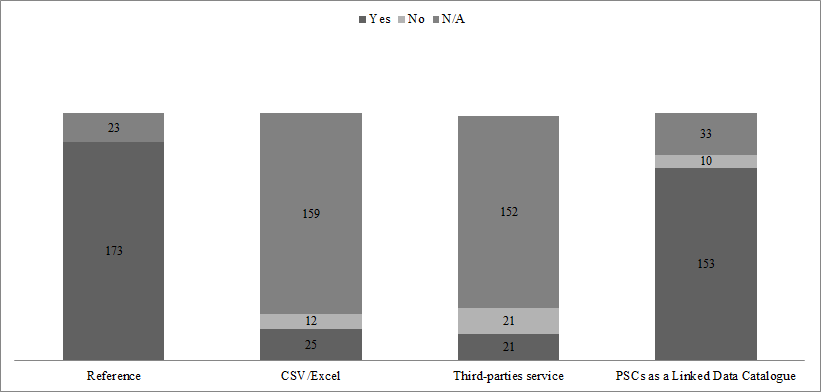
\includegraphics[width=\textwidth]{./imgs/fig-3}
 \caption{Evolution of the number of terms when a new PSC is linked to the CPV 2008 .}
 \label{fig:results-3}
\end{figure}


\subsection{Study 2}
The aim of this study is to verify if the Linked Data coming from public procurement notices, PSCs, etc. can be consumed to deliver a decision support system that help expert 
users to select CPV codes from user queries in natural language. This study is motivated by the company Euroaler.net that sells an alert service for users (companies, etc.) 
that want to tender in specific sectors under a certain profile. Usually, the most relevant variables in public procurement notices are the CPV codes and the 
location (NUTS codes). In this experiment we simulate the behavior of Euroalert.net employees when they have to translate user queries into CPV codes 
for creating a new alert. Basically, the experiment is based on traditional semantic search and concept query expansion methods that we have designed to 
tackle the recommendation of CPV codes, see. Table~\ref{methods-recommending} . 


\subsection{Research Design}


\begin{table}[!htb]
\renewcommand{\arraystretch}{1.3}
\begin{center}
\begin{tabular}[c]{|l|p{8.5cm}|p{4.5cm}|} 
\hline
\textbf{Method} &  \textbf{Description} &  \textbf{Technology} \\\hline
$M^1$ & CPV English descriptions are indexed and a syntactic search process is performed for each $Q_i$ & Apache Lucene y Solr \\ \hline
$M^2$ & CPV codes are selected according to the SKOS taxonomy. Previously, the method $M^1$ is applied to extract CPV codes from natural language & $M^1$ + ranking broader/narrower \\ \hline
$M^3$ & Similar to $M^2$ but codes are selected using \textit{Spreading Activation}& $M^1$ + ONTOSPREAD \\ \hline
$M^4$ & Similar to $M^2$ but codes are selected using the analysis of historical relationships in previous public procurement notices & $M^1$ + Apache Mahout \\ \hline
 \end{tabular}
  \caption{Methods for recommending CPV 2008 codes.}\label{methods-recommending}  
    \end{center}
\end{table}


% Since the CORFU approach has been designed and implemented~\footnote{\url{https://github.com/chemaar/corfu}} it is necessary to 
% establish a method to assess quantitatively the quality of the results.  The steps to carry 
% out this experiment are: 1) Configure the CORFU technique, see Table~\ref{config-corfu};  
% 2) Execute the algorithm taking as a parameter the file containing the whole dataset of company names;
% 3) Validate (manually) the dump of unified names; 4) Calculate the measures of 
% precision, see Eq.~\ref{eq-1}, recall, see Eq.~\ref{eq-2}, and the F1 score (the harmonic mean of precision and recall), see Eq.~\ref{eq-3} according to the values of $tp$ (true positive), 
% $fp$ (false positive), $tn$ (true negative) and $fn$ (false negative). In particular, this evaluation considers the precision of the algorithm as ``the number of supplier names that have been correctly unified under the same name'' while recall is 
% ``the number of supplier names that have not been correctly classified under a proper name''.  More specifically, $tp$ is ``the number of corporate names properly unified'', $fp$ is 
% ``the number of corporate names wrongly unified'', $tn$ is ``the number of corporate names properly non-unified'' and $fn$ is ``the number of corporate names wrongly non-unified''.
% 
% 


\begin{figure}[ht]
\begin{minipage}[b]{0.45\linewidth}
\centering
\begin{equation}\label{eq-1}
Precision = \frac{tp}{tp+fp} 
\end{equation}
\end{minipage}
\hspace{0.5cm}
\begin{minipage}[b]{0.45\linewidth}
\centering
\begin{equation}\label{eq-2}
Recall = \frac{tp}{tp+fn}
\end{equation}
\end{minipage}
\end{figure}


\begin{equation}\label{eq-3}
F1 = 2 \cdot \frac{Precision \cdot Recall}{ Precision + Recall}
\end{equation}




\subsection{Sample}
In order to carry out this study we have used the next samples of data:
\begin{itemize}
\item A dataset of 1 million of public procurement notices provided by Euroalert.net containing CPV and NUTS codes.
\item A set of 11 user queries and the expected CPV codes created by Euroalert.net employees, see Table~\ref{expected-codes} (queries have been ``normalized'' according to one CPV descriptor to keep privacy) .
\item The CPV dataset as Linked Data.
\end{itemize}



\begin{table}[!htb]
\renewcommand{\arraystretch}{1.3}
\begin{center}
\begin{tabular}[c]{|l|p{8.5cm}|p{4cm}|} 
\hline
  \multirow{2}{*}\textbf{$Q_{i}$} &  \textbf{User query-$Q_{str}$} &  \textbf{Number of expected CPV codes-$\#Q^{i}_{cpv}$} \\\hline
  $Q_1$ & ``Comprehensive overview over all environmental technologies renewable energy products'' & $463$ \\ \hline
  $Q_2$ & ``Tendering of public works: housing, hospitals, roads, housing developments, station drinking water treatment, reforestation'' & $35$ \\ \hline
  $Q_3$ & ``Prefabricated buildings'' & $7$ \\ \hline
  $Q_4$ & ``Games for children (parks swings, slides, land of play equipment in the public sphere'' & $26$ \\ \hline
  $Q_5$ & ``Vital signs monitor'' &  $277$\\ \hline
  $Q_6$ & ``Museum and exhibition and product launch services'' & $1$ \\ \hline
  $Q_7$ & ``Voltmeters, instruments measuring electrical quantities, Ammeters, Instruments for checking physical characteristics, hygrometers, thermometers, measuring equipment and control, leak detector, Analyzers, 
  Cable Splicing insulated cable joints kits, screwdrivers, hand tools , screwdriver'' & $117$ \\ \hline
  $Q_8$ & ``Conservation Maintenance of pavements for roads, airfields, bridges, tunnels'' & $13$ \\ \hline
  $Q_9$ & ``Wood poles, Wooden sleepers , Lattice towers'' & $10$ \\ \hline
  $Q_{10}$ & ``Architectural, construction, engineering and inspection services'' &  $173$\\ \hline
  $Q_{11}$ & ``Medical practice and related services'' &  $13$\\ \hline
 \end{tabular}
  \caption{User queries and number of expected CPV codes.}\label{expected-codes}  
    \end{center}
\end{table}




\subsection{Results and Discussion}
According to the results in Table~\ref{table:queries-ir-results}, the method that better match the behavior of an expert user is $M^1$ followed by $M^3$. 
This implies that a method based on natural language processing techniques is the most appropriate to translate user queries into CPV codes. 
Oddly, the results of semantic-based methods, $M^2$ and $M^3$, do not get a good performance. Likely, the type of translation 
that the expert user does is more close to a direct language translation than a real thinking about the 
relationships in the taxonomy. Finally, the exploitation of the historical statistics using Apache Mahout algorithms 
(after different iterations and tests we have chosen the best one based on collaborative filtering) do not seem to reflect 
the expert user behavior. Although search and recommendation should not be compared it is strange than a dataset containing the use 
CPV codes in $1$ million public procurement notices could not improve the traditional syntactic search. Nevertheless, there is an 
open issue that lies in the number of true negative codes that in a second step should be validated by experts. 
Thus, the semantic-based methods could improve their results with regards to the traditional one. 



\begin{table}[!htb]
\renewcommand{\arraystretch}{1.3}
\begin{center}
\scriptsize
\begin{tabular}{|c||c|c|c||c|c|c||c|c|c||c|c|c|}
\hline
 \textbf{$M^i$}&\multicolumn{3}{|c||}{$M^{1}$} & \multicolumn{3}{|c||}{$M^{2}$}& \multicolumn{3}{|c||}{$M^{3}$} & \multicolumn{3}{|c|}{$M^{4}$} \\ \hline
\textbf{$Q_i$}/Metric	  &\textbf{P} & \textbf{R} & \textbf{F1} & \textbf{P} & \textbf{R} & \textbf{F1} & \textbf{P} & \textbf{R} & \textbf{F1} & \textbf{P} & \textbf{R} & \textbf{F1}  \\ \hline \hline
$Q_1$  	  &$0,15$ & $0,08$ & $0,10$ &		$0,15$ & $0,15$ & $0,15$ &	$0,12$ & $0,06$ & $0,08$ &	$0,06$ & $0,06$ & $0,06$ \\ \hline
$Q_2$  	  &$0,09$ & $0,09$ & $0,09$ & 		$0,06$ & $0,06$ & $0,06$ & 	$0,03$ & $0,03$ & $0,03$ & 	$0,03$ & $0,03$ & $0,03$ \\ \hline
$Q_3$  	  &$0,14$ & $0,14$ & $0,14$ & 		$0,14$ & $0,14$ & $0,14$ & 	$0,14$ & $0,14$ & $0,14$ & 	$0$ & $0$ & $0$ \\ \hline
$Q_4$  	  &$0,19$ & $0,19$ & $0,19$ &		$0$ 	& $0$ & $0$ & 		$0,12$ & $0,12$ & $0,12$ & 	$0$ & $0$ & $0$ \\ \hline
$Q_5$  	  &$0,12$ & $0,01$ & $0,02$ & 		$0,01$ & $0,01$ & $0,01$ & 	$0,08$ & $0,01$ & $0,02$ & 	$0,03$ & $0,03$ & $0,03$ \\ \hline
$Q_6$  	  &$1,00$ & $1,00$ & $1,00$ & 		$0$ & $0$ & $0$ & 		$1,00$ & $1,00$ & $1,00$ & 	$0,10$ & $0,67$ & $0,17$ \\ \hline
$Q_7$  	  &$0,20$ & $0,20$ & $0,20$ & 		$0,09$ & $0,09$ & $0,09$ & 	$0,15$ & $0,16$ & $0,15$ & 	$0,03$ & $0,03$ & $0,03$ \\ \hline
$Q_8$  	  &$0,08$ & $0,08$ & $0,08$ & 		$0,08$ & $0,08$ & $0,08$ & 	$0,08$ & $0,08$ & $0,08$ & 	$0$ & $0$ & $0$ \\ \hline
$Q_9$  	  &$0,50$ & $0,50$ & $0,50$ & 		$0$ & $0$ & $0$ & 		$0,30$ & $0,38$ & $0,34$ & 	$0$ & $0$ & $0$ \\ \hline
$Q_{10}$  &$0,39$ & $0,39$ & $0,39$ & 		$0,42$ & $0,42$ & $0,42$ & 	$0,34$ & $0,35$ & $0,34$ & 	$0,16$ & $0,16$ & $0,16$ \\ \hline
$Q_{11}$  &$0,23$ & $0,23$ & $0,23$ & 		$0,23$ & $0,23$ & $0,23$ & 	$0,15$ & $0,17$ & $0,16$ & 	$0$ & $0$ & $0$ \\ \hline
\multicolumn{13}{|c|}{\textbf{Average of quanitative measures}} \\ \hline
\textbf{Total}  &$0,28$ & $0,26$ & $0,27$ & 	$0,11$ & $0,11$ & $0,11$ &  	$0,23$ & $0,23$ & $0,224$ &  	$0,03$ & $0,03$ & $0,044$ \\ \hline
\hline
 \end{tabular}
\caption{Quantitative measures (P-precision and R-recall) of methods for recommending CPV codes.}\label{table:queries-ir-results}
  \end{center}
\end{table} 


% \begin{table}[!htb]
% \renewcommand{\arraystretch}{1.3}
% \begin{center}
% \begin{tabular}[c]{|l|c|c|c|} 
% \hline
% \textbf{Method} &  \textbf{Precision} &  \textbf{Recall} & \textbf{F1 score} \\\hline
% $M^1$ & $0.28$ & $0.26$ & $0.26$ \\ \hline
% $M^2$ & $0.11$ & $0.11$ & $0.11$ \\ \hline
% $M^3$ & $0.23$ & $0.23$ & $0.23$ \\ \hline
% $M^4$ & $0.03$ & $0.03$ & $0.03$ \\ \hline
%  \end{tabular}
%   \caption{Quantitative measures (average) of methods for recommending CPV codes.}\label{methods-result}  
%     \end{center}
% \end{table}


